\documentclass[11pt,a4paper,oneside]{report}   
\usepackage{listings}
\linespread{1.5}
%%%%%%%%%%%%%%%%%%%%%%%%%%%%%%%%%
% PACKAGE IMPORTS
%%%%%%%%%%%%%%%%%%%%%%%%%%%%%%%%%


\usepackage[tmargin=2cm,rmargin=1in,lmargin=1in,margin=0.85in,bmargin=2cm,footskip=.2in]{geometry}
\usepackage{amsmath,amsfonts,amsthm,amssymb,mathtools}
\usepackage[varbb]{newpxmath}
\usepackage{xfrac}
\usepackage[makeroom]{cancel}
\usepackage{mathtools}
\usepackage{bookmark}
\usepackage{enumitem}
\usepackage{hyperref,theoremref}
\hypersetup{
	pdftitle={Assignment},
	colorlinks=true, linkcolor=doc!90,
	bookmarksnumbered=true,
	bookmarksopen=true
}
\usepackage[most,many,breakable]{tcolorbox}
\usepackage{xcolor}
\usepackage{varwidth}
\usepackage{varwidth}
\usepackage{etoolbox}
%\usepackage{authblk}
\usepackage{nameref}
\usepackage{multicol,array}
\usepackage{tikz-cd}
\usepackage[ruled,vlined,linesnumbered]{algorithm2e}
\usepackage{comment} % enables the use of multi-line comments (\ifx \fi) 
\usepackage{import}
\usepackage{xifthen}
\usepackage{pdfpages}
\usepackage{transparent}

\newcommand\mycommfont[1]{\footnotesize\ttfamily\textcolor{blue}{#1}}
\SetCommentSty{mycommfont}
\newcommand{\incfig}[1]{%
	\def\svgwidth{\columnwidth}
	\import{./figures/}{#1.pdf_tex}
}

\usepackage{tikzsymbols}
\renewcommand\qedsymbol{$\Laughey$}


%\usepackage{import}
%\usepackage{xifthen}
%\usepackage{pdfpages}
%\usepackage{transparent}


%%%%%%%%%%%%%%%%%%%%%%%%%%%%%%
% SELF MADE COLORS
%%%%%%%%%%%%%%%%%%%%%%%%%%%%%%



\definecolor{myg}{RGB}{56, 140, 70}
\definecolor{myb}{RGB}{45, 111, 177}
\definecolor{myr}{RGB}{199, 68, 64}
\definecolor{mytheorembg}{HTML}{F2F2F9}
\definecolor{mytheoremfr}{HTML}{00007B}
\definecolor{mylenmabg}{HTML}{FFFAF8}
\definecolor{mylenmafr}{HTML}{983b0f}
\definecolor{mypropbg}{HTML}{f2fbfc}
\definecolor{mypropfr}{HTML}{191971}
\definecolor{myexamplebg}{HTML}{F2FBF8}
\definecolor{myexamplefr}{HTML}{88D6D1}
\definecolor{myexampleti}{HTML}{2A7F7F}
\definecolor{mydefinitbg}{HTML}{E5E5FF}
\definecolor{mydefinitfr}{HTML}{3F3FA3}
\definecolor{notesgreen}{RGB}{0,162,0}
\definecolor{myp}{RGB}{197, 92, 212}
\definecolor{mygr}{HTML}{2C3338}
\definecolor{myred}{RGB}{127,0,0}
\definecolor{myyellow}{RGB}{169,121,69}
\definecolor{myexercisebg}{HTML}{F2FBF8}
\definecolor{myexercisefg}{HTML}{88D6D1}


%%%%%%%%%%%%%%%%%%%%%%%%%%%%
% TCOLORBOX SETUPS
%%%%%%%%%%%%%%%%%%%%%%%%%%%%

\setlength{\parindent}{1cm}
%================================
% THEOREM BOX
%================================

\tcbuselibrary{theorems,skins,hooks}
\newtcbtheorem[number within=section]{Theorem}{Theorem}
{%
	enhanced,
	breakable,
	colback = mytheorembg,
	frame hidden,
	boxrule = 0sp,
	borderline west = {2pt}{0pt}{mytheoremfr},
	sharp corners,
	detach title,
	before upper = \tcbtitle\par\smallskip,
	coltitle = mytheoremfr,
	fonttitle = \bfseries\sffamily,
	description font = \mdseries,
	separator sign none,
	segmentation style={solid, mytheoremfr},
}
{th}

\tcbuselibrary{theorems,skins,hooks}
\newtcbtheorem[number within=chapter]{theorem}{Theorem}
{%
	enhanced,
	breakable,
	colback = mytheorembg,
	frame hidden,
	boxrule = 0sp,
	borderline west = {2pt}{0pt}{mytheoremfr},
	sharp corners,
	detach title,
	before upper = \tcbtitle\par\smallskip,
	coltitle = mytheoremfr,
	fonttitle = \bfseries\sffamily,
	description font = \mdseries,
	separator sign none,
	segmentation style={solid, mytheoremfr},
}
{th}


\tcbuselibrary{theorems,skins,hooks}
\newtcolorbox{Theoremcon}
{%
	enhanced
	,breakable
	,colback = mytheorembg
	,frame hidden
	,boxrule = 0sp
	,borderline west = {2pt}{0pt}{mytheoremfr}
	,sharp corners
	,description font = \mdseries
	,separator sign none
}

%================================
% Corollery
%================================
\tcbuselibrary{theorems,skins,hooks}
\newtcbtheorem[number within=section]{Corollary}{Corollary}
{%
	enhanced
	,breakable
	,colback = myp!10
	,frame hidden
	,boxrule = 0sp
	,borderline west = {2pt}{0pt}{myp!85!black}
	,sharp corners
	,detach title
	,before upper = \tcbtitle\par\smallskip
	,coltitle = myp!85!black
	,fonttitle = \bfseries\sffamily
	,description font = \mdseries
	,separator sign none
	,segmentation style={solid, myp!85!black}
}
{th}
\tcbuselibrary{theorems,skins,hooks}
\newtcbtheorem[number within=chapter]{corollary}{Corollary}
{%
	enhanced
	,breakable
	,colback = myp!10
	,frame hidden
	,boxrule = 0sp
	,borderline west = {2pt}{0pt}{myp!85!black}
	,sharp corners
	,detach title
	,before upper = \tcbtitle\par\smallskip
	,coltitle = myp!85!black
	,fonttitle = \bfseries\sffamily
	,description font = \mdseries
	,separator sign none
	,segmentation style={solid, myp!85!black}
}
{th}


%================================
% LENMA
%================================

\tcbuselibrary{theorems,skins,hooks}
\newtcbtheorem[number within=section]{Lenma}{Lenma}
{%
	enhanced,
	breakable,
	colback = mylenmabg,
	frame hidden,
	boxrule = 0sp,
	borderline west = {2pt}{0pt}{mylenmafr},
	sharp corners,
	detach title,
	before upper = \tcbtitle\par\smallskip,
	coltitle = mylenmafr,
	fonttitle = \bfseries\sffamily,
	description font = \mdseries,
	separator sign none,
	segmentation style={solid, mylenmafr},
}
{th}

\tcbuselibrary{theorems,skins,hooks}
\newtcbtheorem[number within=chapter]{lenma}{Lenma}
{%
	enhanced,
	breakable,
	colback = mylenmabg,
	frame hidden,
	boxrule = 0sp,
	borderline west = {2pt}{0pt}{mylenmafr},
	sharp corners,
	detach title,
	before upper = \tcbtitle\par\smallskip,
	coltitle = mylenmafr,
	fonttitle = \bfseries\sffamily,
	description font = \mdseries,
	separator sign none,
	segmentation style={solid, mylenmafr},
}
{th}


%================================
% PROPOSITION
%================================

\tcbuselibrary{theorems,skins,hooks}
\newtcbtheorem[number within=section]{Prop}{Proposition}
{%
	enhanced,
	breakable,
	colback = mypropbg,
	frame hidden,
	boxrule = 0sp,
	borderline west = {2pt}{0pt}{mypropfr},
	sharp corners,
	detach title,
	before upper = \tcbtitle\par\smallskip,
	coltitle = mypropfr,
	fonttitle = \bfseries\sffamily,
	description font = \mdseries,
	separator sign none,
	segmentation style={solid, mypropfr},
}
{th}

\tcbuselibrary{theorems,skins,hooks}
\newtcbtheorem[number within=chapter]{prop}{Proposition}
{%
	enhanced,
	breakable,
	colback = mypropbg,
	frame hidden,
	boxrule = 0sp,
	borderline west = {2pt}{0pt}{mypropfr},
	sharp corners,
	detach title,
	before upper = \tcbtitle\par\smallskip,
	coltitle = mypropfr,
	fonttitle = \bfseries\sffamily,
	description font = \mdseries,
	separator sign none,
	segmentation style={solid, mypropfr},
}
{th}


%================================
% CLAIM
%================================

\tcbuselibrary{theorems,skins,hooks}
\newtcbtheorem[number within=section]{claim}{Claim}
{%
	enhanced
	,breakable
	,colback = myg!10
	,frame hidden
	,boxrule = 0sp
	,borderline west = {2pt}{0pt}{myg}
	,sharp corners
	,detach title
	,before upper = \tcbtitle\par\smallskip
	,coltitle = myg!85!black
	,fonttitle = \bfseries\sffamily
	,description font = \mdseries
	,separator sign none
	,segmentation style={solid, myg!85!black}
}
{th}



%================================
% Exercise
%================================

\tcbuselibrary{theorems,skins,hooks}
\newtcbtheorem[number within=section]{Exercise}{Exercise}
{%
	enhanced,
	breakable,
	colback = myexercisebg,
	frame hidden,
	boxrule = 0sp,
	borderline west = {2pt}{0pt}{myexercisefg},
	sharp corners,
	detach title,
	before upper = \tcbtitle\par\smallskip,
	coltitle = myexercisefg,
	fonttitle = \bfseries\sffamily,
	description font = \mdseries,
	separator sign none,
	segmentation style={solid, myexercisefg},
}
{th}

\tcbuselibrary{theorems,skins,hooks}
\newtcbtheorem[number within=chapter]{exercise}{Exercise}
{%
	enhanced,
	breakable,
	colback = myexercisebg,
	frame hidden,
	boxrule = 0sp,
	borderline west = {2pt}{0pt}{myexercisefg},
	sharp corners,
	detach title,
	before upper = \tcbtitle\par\smallskip,
	coltitle = myexercisefg,
	fonttitle = \bfseries\sffamily,
	description font = \mdseries,
	separator sign none,
	segmentation style={solid, myexercisefg},
}
{th}

%================================
% EXAMPLE BOX
%================================

\newtcbtheorem[number within=section]{Example}{Example}
{%
	colback = myexamplebg
	,breakable
	,colframe = myexamplefr
	,coltitle = myexampleti
	,boxrule = 1pt
	,sharp corners
	,detach title
	,before upper=\tcbtitle\par\smallskip
	,fonttitle = \bfseries
	,description font = \mdseries
	,separator sign none
	,description delimiters parenthesis
}
{ex}

\newtcbtheorem[number within=chapter]{example}{Example}
{%
	colback = myexamplebg
	,breakable
	,colframe = myexamplefr
	,coltitle = myexampleti
	,boxrule = 1pt
	,sharp corners
	,detach title
	,before upper=\tcbtitle\par\smallskip
	,fonttitle = \bfseries
	,description font = \mdseries
	,separator sign none
	,description delimiters parenthesis
}
{ex}

%================================
% DEFINITION BOX
%================================

\newtcbtheorem[number within=section]{Definition}{Definition}{enhanced,
	before skip=2mm,after skip=2mm, colback=red!5,colframe=red!80!black,boxrule=0.5mm,
	attach boxed title to top left={xshift=1cm,yshift*=1mm-\tcboxedtitleheight}, varwidth boxed title*=-3cm,
	boxed title style={frame code={
					\path[fill=tcbcolback]
					([yshift=-1mm,xshift=-1mm]frame.north west)
					arc[start angle=0,end angle=180,radius=1mm]
					([yshift=-1mm,xshift=1mm]frame.north east)
					arc[start angle=180,end angle=0,radius=1mm];
					\path[left color=tcbcolback!60!black,right color=tcbcolback!60!black,
						middle color=tcbcolback!80!black]
					([xshift=-2mm]frame.north west) -- ([xshift=2mm]frame.north east)
					[rounded corners=1mm]-- ([xshift=1mm,yshift=-1mm]frame.north east)
					-- (frame.south east) -- (frame.south west)
					-- ([xshift=-1mm,yshift=-1mm]frame.north west)
					[sharp corners]-- cycle;
				},interior engine=empty,
		},
	fonttitle=\bfseries,
	title={#2},#1}{def}
\newtcbtheorem[number within=chapter]{definition}{Definition}{enhanced,
	before skip=2mm,after skip=2mm, colback=red!5,colframe=red!80!black,boxrule=0.5mm,
	attach boxed title to top left={xshift=1cm,yshift*=1mm-\tcboxedtitleheight}, varwidth boxed title*=-3cm,
	boxed title style={frame code={
					\path[fill=tcbcolback]
					([yshift=-1mm,xshift=-1mm]frame.north west)
					arc[start angle=0,end angle=180,radius=1mm]
					([yshift=-1mm,xshift=1mm]frame.north east)
					arc[start angle=180,end angle=0,radius=1mm];
					\path[left color=tcbcolback!60!black,right color=tcbcolback!60!black,
						middle color=tcbcolback!80!black]
					([xshift=-2mm]frame.north west) -- ([xshift=2mm]frame.north east)
					[rounded corners=1mm]-- ([xshift=1mm,yshift=-1mm]frame.north east)
					-- (frame.south east) -- (frame.south west)
					-- ([xshift=-1mm,yshift=-1mm]frame.north west)
					[sharp corners]-- cycle;
				},interior engine=empty,
		},
	fonttitle=\bfseries,
	title={#2},#1}{def}



%================================
% Solution BOX
%================================

\makeatletter
\newtcbtheorem{question}{Question}{enhanced,
	breakable,
	colback=white,
	colframe=myb!80!black,
	attach boxed title to top left={yshift*=-\tcboxedtitleheight},
	fonttitle=\bfseries,
	title={#2},
	boxed title size=title,
	boxed title style={%
			sharp corners,
			rounded corners=northwest,
			colback=tcbcolframe,
			boxrule=0pt,
		},
	underlay boxed title={%
			\path[fill=tcbcolframe] (title.south west)--(title.south east)
			to[out=0, in=180] ([xshift=5mm]title.east)--
			(title.center-|frame.east)
			[rounded corners=\kvtcb@arc] |-
			(frame.north) -| cycle;
		},
	#1
}{def}
\makeatother

%================================
% SOLUTION BOX
%================================

\makeatletter
\newtcolorbox{solution}{enhanced,
	breakable,
	colback=white,
	colframe=myg!80!black,
	attach boxed title to top left={yshift*=-\tcboxedtitleheight},
	title=Solution,
	boxed title size=title,
	boxed title style={%
			sharp corners,
			rounded corners=northwest,
			colback=tcbcolframe,
			boxrule=0pt,
		},
	underlay boxed title={%
			\path[fill=tcbcolframe] (title.south west)--(title.south east)
			to[out=0, in=180] ([xshift=5mm]title.east)--
			(title.center-|frame.east)
			[rounded corners=\kvtcb@arc] |-
			(frame.north) -| cycle;
		},
}
\makeatother

%================================
% Question BOX
%================================

\makeatletter
\newtcbtheorem{qstion}{Question}{enhanced,
	breakable,
	colback=white,
	colframe=mygr,
	attach boxed title to top left={yshift*=-\tcboxedtitleheight},
	fonttitle=\bfseries,
	title={#2},
	boxed title size=title,
	boxed title style={%
			sharp corners,
			rounded corners=northwest,
			colback=tcbcolframe,
			boxrule=0pt,
		},
	underlay boxed title={%
			\path[fill=tcbcolframe] (title.south west)--(title.south east)
			to[out=0, in=180] ([xshift=5mm]title.east)--
			(title.center-|frame.east)
			[rounded corners=\kvtcb@arc] |-
			(frame.north) -| cycle;
		},
	#1
}{def}
\makeatother

\newtcbtheorem[number within=chapter]{wconc}{Wrong Concept}{
	breakable,
	enhanced,
	colback=white,
	colframe=myr,
	arc=0pt,
	outer arc=0pt,
	fonttitle=\bfseries\sffamily\large,
	colbacktitle=myr,
	attach boxed title to top left={},
	boxed title style={
			enhanced,
			skin=enhancedfirst jigsaw,
			arc=3pt,
			bottom=0pt,
			interior style={fill=myr}
		},
	#1
}{def}



%================================
% NOTE BOX
%================================

\usetikzlibrary{arrows,calc,shadows.blur}
\tcbuselibrary{skins}
\newtcolorbox{note}[1][]{%
	enhanced jigsaw,
	colback=gray!20!white,%
	colframe=gray!80!black,
	size=small,
	boxrule=1pt,
	title=\textbf{Note:-},
	halign title=flush center,
	coltitle=black,
	breakable,
	drop shadow=black!50!white,
	attach boxed title to top left={xshift=1cm,yshift=-\tcboxedtitleheight/2,yshifttext=-\tcboxedtitleheight/2},
	minipage boxed title=1.5cm,
	boxed title style={%
			colback=white,
			size=fbox,
			boxrule=1pt,
			boxsep=2pt,
			underlay={%
					\coordinate (dotA) at ($(interior.west) + (-0.5pt,0)$);
					\coordinate (dotB) at ($(interior.east) + (0.5pt,0)$);
					\begin{scope}
						\clip (interior.north west) rectangle ([xshift=3ex]interior.east);
						\filldraw [white, blur shadow={shadow opacity=60, shadow yshift=-.75ex}, rounded corners=2pt] (interior.north west) rectangle (interior.south east);
					\end{scope}
					\begin{scope}[gray!80!black]
						\fill (dotA) circle (2pt);
						\fill (dotB) circle (2pt);
					\end{scope}
				},
		},
	#1,
}

%%%%%%%%%%%%%%%%%%%%%%%%%%%%%%
% SELF MADE COMMANDS
%%%%%%%%%%%%%%%%%%%%%%%%%%%%%%


\newcommand{\thm}[2]{\begin{Theorem}{#1}{}#2\end{Theorem}}
\newcommand{\cor}[2]{\begin{Corollary}{#1}{}#2\end{Corollary}}
\newcommand{\mlenma}[2]{\begin{Lenma}{#1}{}#2\end{Lenma}}
\newcommand{\mprop}[2]{\begin{Prop}{#1}{}#2\end{Prop}}
\newcommand{\clm}[3]{\begin{claim}{#1}{#2}#3\end{claim}}
\newcommand{\wc}[2]{\begin{wconc}{#1}{}\setlength{\parindent}{1cm}#2\end{wconc}}
\newcommand{\thmcon}[1]{\begin{Theoremcon}{#1}\end{Theoremcon}}
\newcommand{\ex}[2]{\begin{Example}{#1}{}#2\end{Example}}
\newcommand{\dfn}[2]{\begin{Definition}[colbacktitle=red!75!black]{#1}{}#2\end{Definition}}
\newcommand{\dfnc}[2]{\begin{definition}[colbacktitle=red!75!black]{#1}{}#2\end{definition}}
\newcommand{\qs}[2]{\begin{question}{#1}{}#2\end{question}}
\newcommand{\pf}[2]{\begin{myproof}[#1]#2\end{myproof}}
\newcommand{\nt}[1]{\begin{note}#1\end{note}}

\newcommand*\circled[1]{\tikz[baseline=(char.base)]{
		\node[shape=circle,draw,inner sep=1pt] (char) {#1};}}
\newcommand\getcurrentref[1]{%
	\ifnumequal{\value{#1}}{0}
	{??}
	{\the\value{#1}}%
}
\newcommand{\getCurrentSectionNumber}{\getcurrentref{section}}
\newenvironment{myproof}[1][\proofname]{%
	\proof[\bfseries #1: ]%
}{\endproof}

\newcommand{\mclm}[2]{\begin{myclaim}[#1]#2\end{myclaim}}
\newenvironment{myclaim}[1][\claimname]{\proof[\bfseries #1: ]}{}

\newcounter{mylabelcounter}

\makeatletter
\newcommand{\setword}[2]{%
	\phantomsection
	#1\def\@currentlabel{\unexpanded{#1}}\label{#2}%
}
\makeatother




\tikzset{
	symbol/.style={
			draw=none,
			every to/.append style={
					edge node={node [sloped, allow upside down, auto=false]{$#1$}}}
		}
}


% deliminators
\DeclarePairedDelimiter{\abs}{\lvert}{\rvert}
\DeclarePairedDelimiter{\norm}{\lVert}{\rVert}

\DeclarePairedDelimiter{\ceil}{\lceil}{\rceil}
\DeclarePairedDelimiter{\floor}{\lfloor}{\rfloor}
\DeclarePairedDelimiter{\round}{\lfloor}{\rceil}

\newsavebox\diffdbox
\newcommand{\slantedromand}{{\mathpalette\makesl{d}}}
\newcommand{\makesl}[2]{%
	\begingroup
	\sbox{\diffdbox}{$\mathsurround=0pt#1\mathrm{#2}$}%
	\pdfsave
	\pdfsetmatrix{1 0 0.2 1}%
	\rlap{\usebox{\diffdbox}}%
	\pdfrestore
	\hskip\wd\diffdbox
	\endgroup
}
\newcommand{\dd}[1][]{\ensuremath{\mathop{}\!\ifstrempty{#1}{%
			\slantedromand\@ifnextchar^{\hspace{0.2ex}}{\hspace{0.1ex}}}%
		{\slantedromand\hspace{0.2ex}^{#1}}}}
\ProvideDocumentCommand\dv{o m g}{%
	\ensuremath{%
		\IfValueTF{#3}{%
			\IfNoValueTF{#1}{%
				\frac{\dd #2}{\dd #3}%
			}{%
				\frac{\dd^{#1} #2}{\dd #3^{#1}}%
			}%
		}{%
			\IfNoValueTF{#1}{%
				\frac{\dd}{\dd #2}%
			}{%
				\frac{\dd^{#1}}{\dd #2^{#1}}%
			}%
		}%
	}%
}
\providecommand*{\pdv}[3][]{\frac{\partial^{#1}#2}{\partial#3^{#1}}}
%  - others
\DeclareMathOperator{\Lap}{\mathcal{L}}
\DeclareMathOperator{\Var}{Var} % varience
\DeclareMathOperator{\Cov}{Cov} % covarience
\DeclareMathOperator{\E}{E} % expected

% Since the amsthm package isn't loaded

% I prefer the slanted \leq
\let\oldleq\leq % save them in case they're every wanted
\let\oldgeq\geq
\renewcommand{\leq}{\leqslant}
\renewcommand{\geq}{\geqslant}

% % redefine matrix env to allow for alignment, use r as default
% \renewcommand*\env@matrix[1][r]{\hskip -\arraycolsep
%     \let\@ifnextchar\new@ifnextchar
%     \array{*\c@MaxMatrixCols #1}}


%\usepackage{framed}
%\usepackage{titletoc}
%\usepackage{etoolbox}
%\usepackage{lmodern}


%\patchcmd{\tableofcontents}{\contentsname}{\sffamily\contentsname}{}{}

%\renewenvironment{leftbar}
%{\def\FrameCommand{\hspace{6em}%
%		{\color{myyellow}\vrule width 2pt depth 6pt}\hspace{1em}}%
%	\MakeFramed{\parshape 1 0cm \dimexpr\textwidth-6em\relax\FrameRestore}\vskip2pt%
%}
%{\endMakeFramed}

%\titlecontents{chapter}
%[0em]{\vspace*{2\baselineskip}}
%{\parbox{4.5em}{%
%		\hfill\Huge\sffamily\bfseries\color{myred}\thecontentspage}%
%	\vspace*{-2.3\baselineskip}\leftbar\textsc{\small\chaptername~\thecontentslabel}\\\sffamily}
%{}{\endleftbar}
%\titlecontents{section}
%[8.4em]
%{\sffamily\contentslabel{3em}}{}{}
%{\hspace{0.5em}\nobreak\itshape\color{myred}\contentspage}
%\titlecontents{subsection}
%[8.4em]
%{\sffamily\contentslabel{3em}}{}{}  
%{\hspace{0.5em}\nobreak\itshape\color{myred}\contentspage}



%%%%%%%%%%%%%%%%%%%%%%%%%%%%%%%%%%%%%%%%%%%
% TABLE OF CONTENTS
%%%%%%%%%%%%%%%%%%%%%%%%%%%%%%%%%%%%%%%%%%%

\usepackage{tikz}
\definecolor{doc}{RGB}{0,60,110}
\usepackage{titletoc}
\contentsmargin{0cm}
\titlecontents{chapter}[3.7pc]
{\addvspace{30pt}%
	\begin{tikzpicture}[remember picture, overlay]%
		\draw[fill=doc!60,draw=doc!60] (-7,-.1) rectangle (-0.9,.5);%
		\pgftext[left,x=-3.5cm,y=0.2cm]{\color{white}\Large\sc\bfseries Chapter\ \thecontentslabel};%
	\end{tikzpicture}\color{doc!60}\large\sc\bfseries}%
{}
{}
{\;\titlerule\;\large\sc\bfseries Page \thecontentspage
	\begin{tikzpicture}[remember picture, overlay]
		\draw[fill=doc!60,draw=doc!60] (2pt,0) rectangle (4,0.1pt);
	\end{tikzpicture}}%
\titlecontents{section}[3.7pc]
{\addvspace{2pt}}
{\contentslabel[\thecontentslabel]{2pc}}
{}
{\hfill\small \thecontentspage}
[]
\titlecontents*{subsection}[3.7pc]
{\addvspace{-1pt}\small}
{}
{}
{\ --- \small\thecontentspage}
[ \textbullet\ ][]

\makeatletter
\renewcommand{\tableofcontents}{%
	\chapter*{%
	  \vspace*{-20\p@}%
	  \begin{tikzpicture}[remember picture, overlay]%
		  \pgftext[right,x=15cm,y=0.2cm]{\color{doc!60}\Huge\sc\bfseries \contentsname};%
		  \draw[fill=doc!60,draw=doc!60] (13,-.75) rectangle (20,1);%
		  \clip (13,-.75) rectangle (20,1);
		  \pgftext[right,x=15cm,y=0.2cm]{\color{white}\Huge\sc\bfseries \contentsname};%
	  \end{tikzpicture}}%
	\@starttoc{toc}}
\makeatother


\usepackage{graphicx}
\graphicspath{ {./images/} }

\title{\Huge{MSc - Media and Textmining}\\Homework results}
\author{\huge{Daniel Mark Kiss}}
\date{2023}

\begin{document}

\maketitle
\newpage
\tableofcontents
\pagebreak

\chapter{Introduction}

Amazon Web Services (AWS) is a comprehensive cloud computing platform provided by Amazon. It includes a mixture of infrastructure-as-a-service (IaaS), platform-as-a-service (PaaS) and packaged-software-as-a-service (SaaS). It offers a vast array of cloud services, including computing power, storage, databases, machine learning, analytics, and more. AWS allows individuals and organizations to access and utilize computing resources over the internet, without the need to own or maintain physical servers and infrastructure.
Amazon launched its first web services in 2002 from the internal infrastructure that Amazon.com built to handle its online retail operations. In 2006, it began offering its defining IaaS services. AWS was one of the first companies to introduce a pay-as-you-go cloud computing model that scales to provide users with compute, storage or throughput as needed.
AWS is separated into different services; each can be configured in different ways based on the user's needs. Users can see configuration options and individual server maps for an AWS service. AWS provides a scalable and flexible environment for businesses to build, deploy, and manage applications and services. It offers a pay-as-you-go pricing model, which means users only pay for the resources they consume, making it cost-effective and efficient for a wide range of use cases. \cite{techtagaws}

\chapter{Current AWS features and techologies}

Before I started the development of the application I have done a course provided by Amazon. It conatains a 14 module class where they teache the fundamentals of AWS.
It was roughly 5 weeks for me to finish and complete all laboratory exercises and module closing quiz. Throughout the course I have familiarised myself with the different AWS services and theoretical background. It proved to be a good repetition for my previous knowledge like REST API.


\section{Amazon Elastic Compute Cloud (EC2)}

This service provides resizable compute capacity in the cloud, allowing users to run virtual servers, known as "instances," for various computing tasks.
Key features:
\begin{enumerate}
  \item Scalability: EC2 instances can be quickly scaled up or down based on demand. This means that users can add or remove instances to match the needs of their applications or workloads.
  \item Variety of Instance Types: EC2 offers a wide range of instance types optimized for different use cases. These include instances optimized for compute-intensive workloads, memory-intensive tasks, storage-optimized applications, and more.
  \item Operating System Flexibility: Users can choose from a variety of operating systems, including various Linux distributions, Microsoft Windows, and others, to run on their EC2 instances.
\end{enumerate}
\section{Amazon Simple Storage Service (S3)}

S3 offers scalable object storage for storing and retrieving data. It is commonly used for data backup, hosting static websites, and as a storage backend for applications.
Amazon S3 is designed to provide durability, availability, and scalability at a low cost.
Key features:
\begin{enumerate}
  \item Object Storage: Amazon S3 stores data as objects, which consist of a file and its associated metadata. Each object is identified by a unique key, making it easy to access and manage.
  \item Buckets: A bucket is a container for objects stored in Amazon S3. Buckets act as top-level folders or directories for organizing and managing objects. Each bucket has a unique name and is associated with a specific AWS region.
  \item Durability and Availability: Amazon S3 is designed to provide 99.999999999% (11 9's) durability for objects over a given year. It achieves this by replicating data across multiple Availability Zones within a region, ensuring high availability.
  \item Scalability: Amazon S3 can scale to accommodate virtually unlimited amounts of data. Users can easily upload, store, and retrieve any amount of data, making it suitable for a wide range of use cases.
  \item ccess Control: Users can control access to their buckets and objects through AWS Identity and Access Management (IAM) policies, bucket policies, Access Control Lists (ACLs), and signed URLs or cookies.
  \item Cross-Region Replication: Users can configure Amazon S3 to automatically replicate objects from one bucket to another in a different AWS region. This helps achieve geographic redundancy and compliance with data residency requirements.
  \item Static Website Hosting: Amazon S3 can be used to host static websites, providing a cost-effective solution for hosting web content.
\end{enumerate}
%\begin{itemize}
%  \item Device tracking
%  \item Raycast
%  \item Plane detection
%  \item Gestures
%  \item Face tracking
%\end{itemize}

\section{Amazon RDS (Relational Database Service)}

RDS offers managed database services for various database engines, including MySQL, PostgreSQL, Oracle, and Microsoft SQL Server.
Key features:
\begin{enumerate}
  \item Managed Service: AWS handles the heavy lifting of database administration tasks such as hardware provisioning, database setup, configuration, patch management, and backups. This allows users to focus on application development rather than database management.
\end{enumerate}

%\begin{figure}[!ht]
%  \centering
%  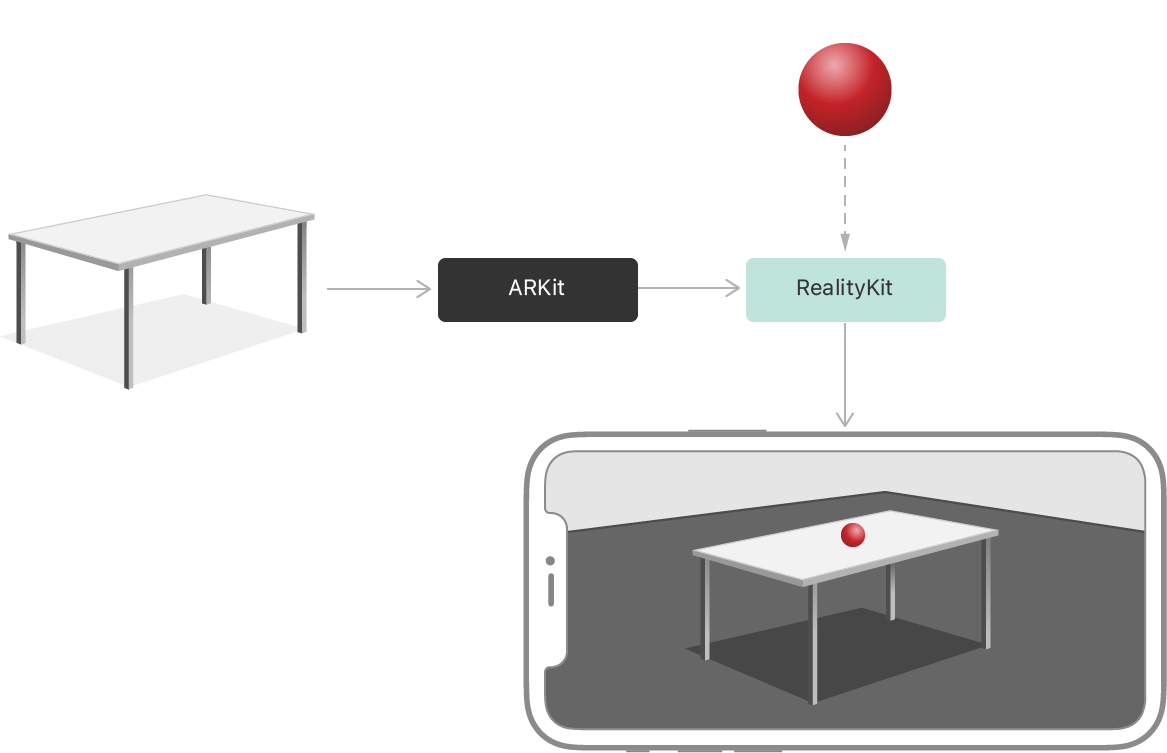
\includegraphics[width=\textwidth]{realitykit.png}
% \includegraphics[width=150mm, keepaspectratio]{figures/TeXnicCenter.png }
%  \caption{RealityKit and ARKit usage.}
%  \label{fig:TexnicCenter}
%\end{figure}

\section{Amazon DynamoDB}

A fully-managed NoSQL database service that provides high performance and seamless scalability for applications that require low-latency access to data.
\begin{enumerate}
  \item NoSQL Database: DynamoDB is a NoSQL database, which means it does not rely on a fixed schema like traditional relational databases. This allows for flexible data modeling, making it well-suited for applications with evolving data structures.
  \item Managed Service: AWS handles all the operational aspects of DynamoDB, including hardware provisioning, setup, configuration, and maintenance. This frees developers from the burden of database management tasks.
  \item Scalability: DynamoDB is designed to scale easily, both in terms of read and write throughput. It can handle massive volumes of traffic and automatically scales based on demand. Users can adjust read and write capacity units to accommodate their application's needs.
\end{enumerate}
\section{AWS Lambda}

This service allows users to run code without provisioning or managing servers. It executes code in response to specific events, making it a key component of serverless architecture.
\begin{enumerate}
  \item Serverless Architecture: Lambda is a serverless computing service, which means developers do not need to manage the underlying servers. Instead, they write code and AWS handles the execution and scaling of that code.
  \item Event-Driven Model: Lambda functions are triggered by events such as changes to data in an Amazon S3 bucket, updates to a DynamoDB table, or incoming HTTP requests via Amazon API Gateway. This event-driven model allows for real-time responses to changes in the environment.
  \item Supported Runtimes: AWS Lambda supports multiple programming languages including Node.js, Python, Java, Go, Ruby, .NET Core, and custom runtimes. This flexibility enables developers to use their preferred programming language.
  \item Pay-per-Use Pricing: With AWS Lambda, users pay only for the compute time consumed by their code. There is no charge when code is not running. This pricing model can lead to cost savings compared to traditional server-based architectures.
\end{enumerate}

\section{AWS CodeCommit}
AWS CodeCommit is a fully managed source control service provided by Amazon Web Services (AWS). It is a secure and scalable Git-based repository hosting service designed to help teams collaborate on code development and version control. CodeCommit provides a secure and reliable platform for storing and managing code repositories.

Key features:
\begin{enumerate}
  \item Git Repository Hosting: CodeCommit supports the Git version control system, providing a familiar interface for developers to manage their code repositories.
  \item Secure and Private: CodeCommit repositories are secure by default and can be configured to be private. Access control policies, AWS Identity and Access Management (IAM) permissions, and encryption options ensure the confidentiality and integrity of code.
  \item Integration with AWS Services: CodeCommit seamlessly integrates with other AWS services, such as AWS CodePipeline, AWS CodeBuild, AWS CodeDeploy, AWS CloudFormation, and more. This enables end-to-end continuous integration and continuous deployment (CI/CD) workflows.
  \item Version Control: CodeCommit allows multiple developers to collaborate on projects by providing version control capabilities. Developers can create branches, merge code changes, and track commit history.
\end{enumerate}


\chapter{Development}

\section{Overview}
For the development phase of the project I used AWS's Cloud9 integrated developer environment(IDE) as the main developer platform for the front-end. For testing I used an iPhone 11 with dual camera system.
I have also version controled the whole development process using git and publishing it on GitHub. Not only the source code can be found there but also the documentation of this project as I have writen it using \LaTeX{}.

\section{APILayer Rest API}

The fundamental part of the application is the data it displays. For retriving the displayed informations I used APILayer's Exchange Rates Data API an open and available for free financial API.  The only problem is that you can only do 250 queries per month in the free version. I used 2 endpoints. The first is '/convert'. With this endpoint, we have any amount conversion from one currency to another. The output of this enpoint is the following JSON.

\begin{lstlisting}[frame=single,float=!ht,caption=JSON from /convert endpoint, label=listing:Bibtex]
  {
    "success": true,
    "query": {
        "from": "EUR",
        "to": "HUF",
        "amount": 1
    },
    "info": {
        "timestamp": 1682930463,
        "rate": 373.180303
    },
    "date": "2023-05-01",
    "result": 373.180303
  }
\end{lstlisting}

The other endpoint used is '/fluctuation'. This endpoint returns the fluctuation data between specified dates. The data can be for all available currencies or for a specific set.
\begin{lstlisting}[frame=single,float=!ht,caption=JSON from /fluctuation endpoint, label=listing:Bibtex]
{
  "base": "EUR",
  "end_date": "2018-02-26",
  "fluctuation": true,
  "rates": {
    "JPY": {
      "change": 0.0635,
      "change_pct": 0.0483,
      "end_rate": 131.651142,
      "start_rate": 131.587611
    },
    "USD": {
      "change": 0.0038,
      "change_pct": 0.3078,
      "end_rate": 1.232735,
      "start_rate": 1.228952
    }
  },
  "start_date": "2018-02-25",
  "success": true
}
\end{lstlisting}

\section{SwiftUI}

SwiftUI is Apple's brand new framework for building user interfaces for iOS, tvOS, macOS, and watchOS. Apple introduced SwiftUI in 2019 and the framework has been evolving ever since. Unlike UIKit, SwiftUI is a cross-platform framework. The key difference with UIKit and AppKit is that SwiftUI defines the user interface declaratively, not imperatively. What does that mean?

Using UIKit you create views to build the view hierarchy of your application's user interface. That is not how SwiftUI works. SwiftUI provides developers with an API to declare or describe what the user interface should look like. SwiftUI inspects the declaration or description of the user interface and converts it to your application's user interface. SwiftUI does the heavy lifting for you.

One of the most challenging aspects of user interface development is synchronizing the application's state and its user interface. Every time the application's state changes, the user interface needs to update to reflect the change. During the development phase, this was a challenge that had to be overcome. Despite the fact that I have already used and developed an iOS application with SwiftUI, it was excellent practice to deepen my knowledge of user state management. I used ObservableObjects to solve this problem.

I used a common state management technique, the MVC pattern, to control the data and model. MVC (Model-View-Controller) is a pattern in software design commonly used to implement user interfaces, data, and controlling logic. It emphasizes a separation between the software's business logic and display. This "separation of concerns" provides for a better division of labor and improved maintenance. Sticking to convention, I created a CurrencyController, CurrencyView and a CurrencyModell class. The CurrencyModel class contains the generated 3D models and their associated values. The task of the CurrencyController class is to query the data and update the information displayed on the View. In the CurrencyView class, it deals with the code defining the appearance of the application and the display of the given dataset.


\section{ARKit and RealityKit}

To operate augmented reality and display the 3D generated graph, I used the ARKit and RealityKit frameworks provided by Apple.

The CurrencyARViewContainer is responsible for displaying the AR view.

\begin{lstlisting}
struct CurrencyARViewContainer: UIViewRepresentable {
    
    @StateObject var controler:CurrencyController
    
    func makeUIView(context: Context) -> ARView{
        AR.view = ARView(frame: .zero)
        return AR.view
    }
    
    func updateUIView(_ uiView: ARView, context: Context) {
        print("updating view - \(controler.timerHappened)")
        uiView.scene.anchors.removeAll()
        ...
    }
}
\end{lstlisting}

To generate the texts and columns, I used the .generateBox() and .generateText() functions of the built-in MeshResource class.
The MeshResource class stores the points defining the shapes. In order for this to become a 3D model, a texture must also be specified. I used the SimpleMaterial() function for this.
We also need an AnchorEntity, which defines the center of our model in the 3D world.
After defining these variables, we can create the ModelEntity and place it in the AR world using the AnchorEntity.

\begin{lstlisting}
    func updateUIView(_ uiView: ARView, context: Context) {
        uiView.scene.anchors.removeAll()
        
        let cylinderMeshResource = MeshResource.generateBox(size: SIMD3(x: 1.2, y: 0.01, z: 0.01), cornerRadius: 0.1)
        
        let myMaterial = SimpleMaterial(color: .gray, roughness: 0, isMetallic: true)
        let radians = 90.0 * Float.pi / 180.0
            
        let kozeppont = AnchorEntity(world: SIMD3(x: 0.0, y: 0.0, z: 0.0))
        let axisXEntity = ModelEntity(mesh: cylinderMeshResource, materials: [myMaterial])
        
        let coneXEntity = ModelEntity(mesh: coneMeshResource, materials: [myMaterial])
        coneXEntity.orientation = simd_quatf(angle: radians, axis: SIMD3(x: 0, y: 0, z: -1))
        
        axisXEntity.addChild(coneXEntity)
        coneXEntity.setPosition(SIMD3(x: 0.6, y: 0.0, z: 0.0), relativeTo: axisXEntity)
        
        
        kozeppont.addChild(axisXEntity)
        uiView.scene.addAnchor(kozeppont)
        ...
    }
\end{lstlisting}

To be able to move the different elements together, all 3D models are children of the axes. Thus, if the axis moves, the connected elements will also move due to the parent-child relationship. In its current version, MeshResource does not support the generation of cones by default, so I was able to achieve this by using an external library package. After importing the RealityGeometries library, I was able to easily generate cones, which I eventually used to draw axes.

\chapter{Presentation of finished work}

In this section I will present and showcase my finished appliction. I will include screenshots to have a better representation and understanding for the reader.
The camera function in the application allows you to capture the current state of the graphs, which in this case came in handy for documentation.


\begin{figure}[!ht]
  \centering
  
\includegraphics[scale=0.2]{front.jpeg}
  % \includegraphics[width=150mm, keepaspectratio]{figures/TeXnicCenter.png}
  \caption{The main screen of the application.}
  \label{fig:TexnicCenter}
\end{figure}

\begin{figure}[!ht]
  \centering
  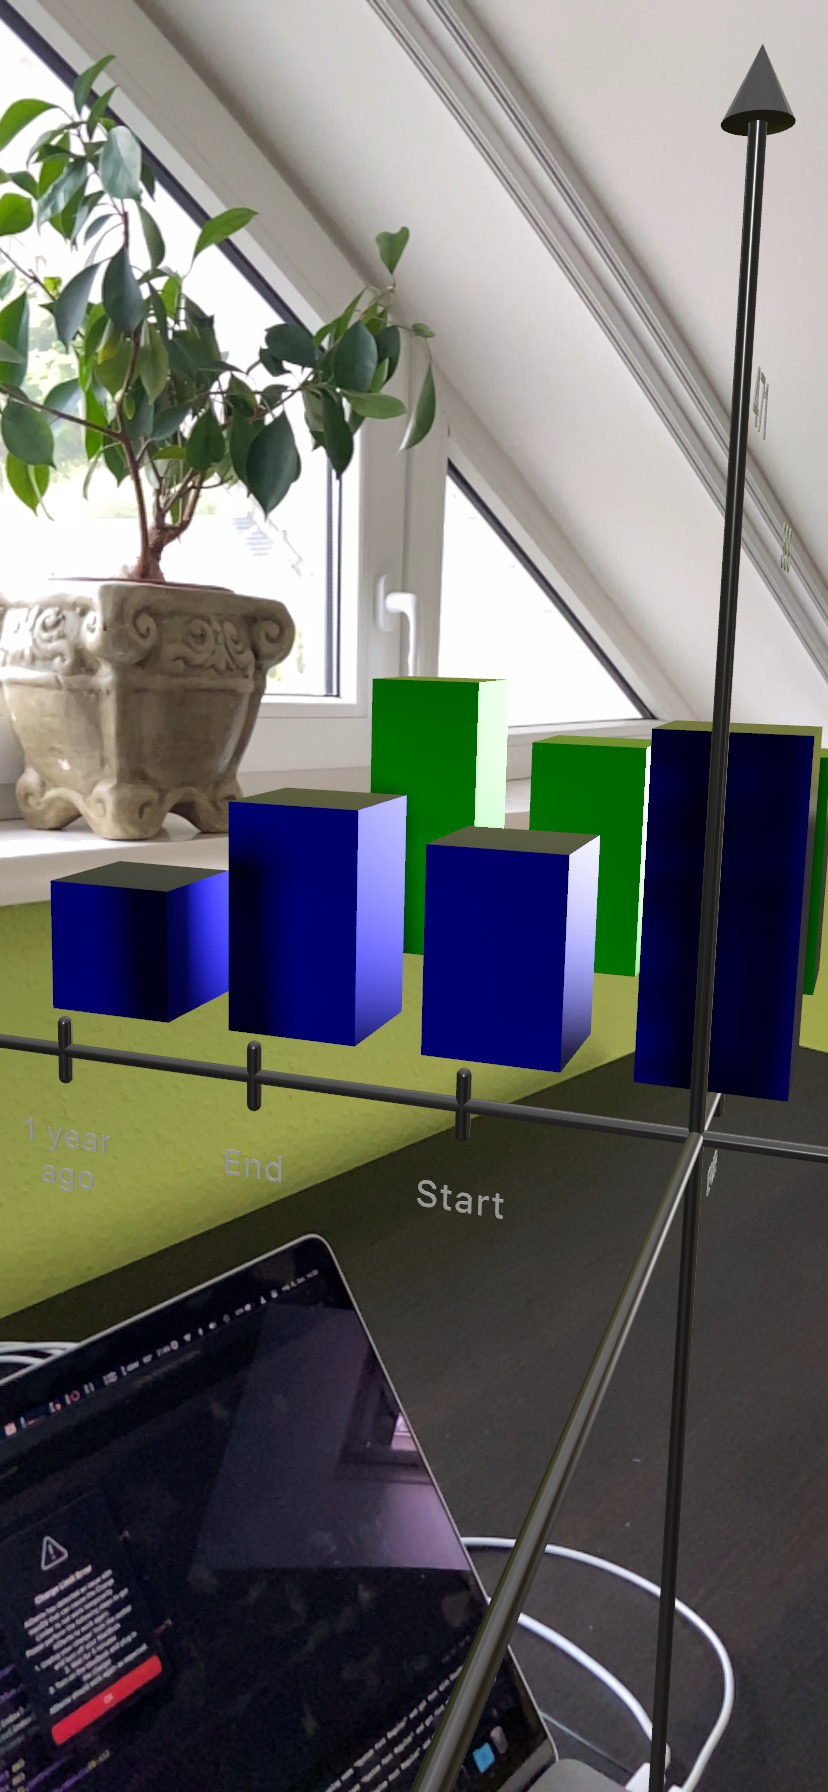
\includegraphics[scale=0.2]{side.jpeg}
  % \includegraphics[width=150mm, keepaspectratio]{figures/TeXnicCenter.png}
  \caption{The main screen of the application.}
  \label{fig:TexnicCenter}
\end{figure}

\begin{figure}[!ht]
  \centering
  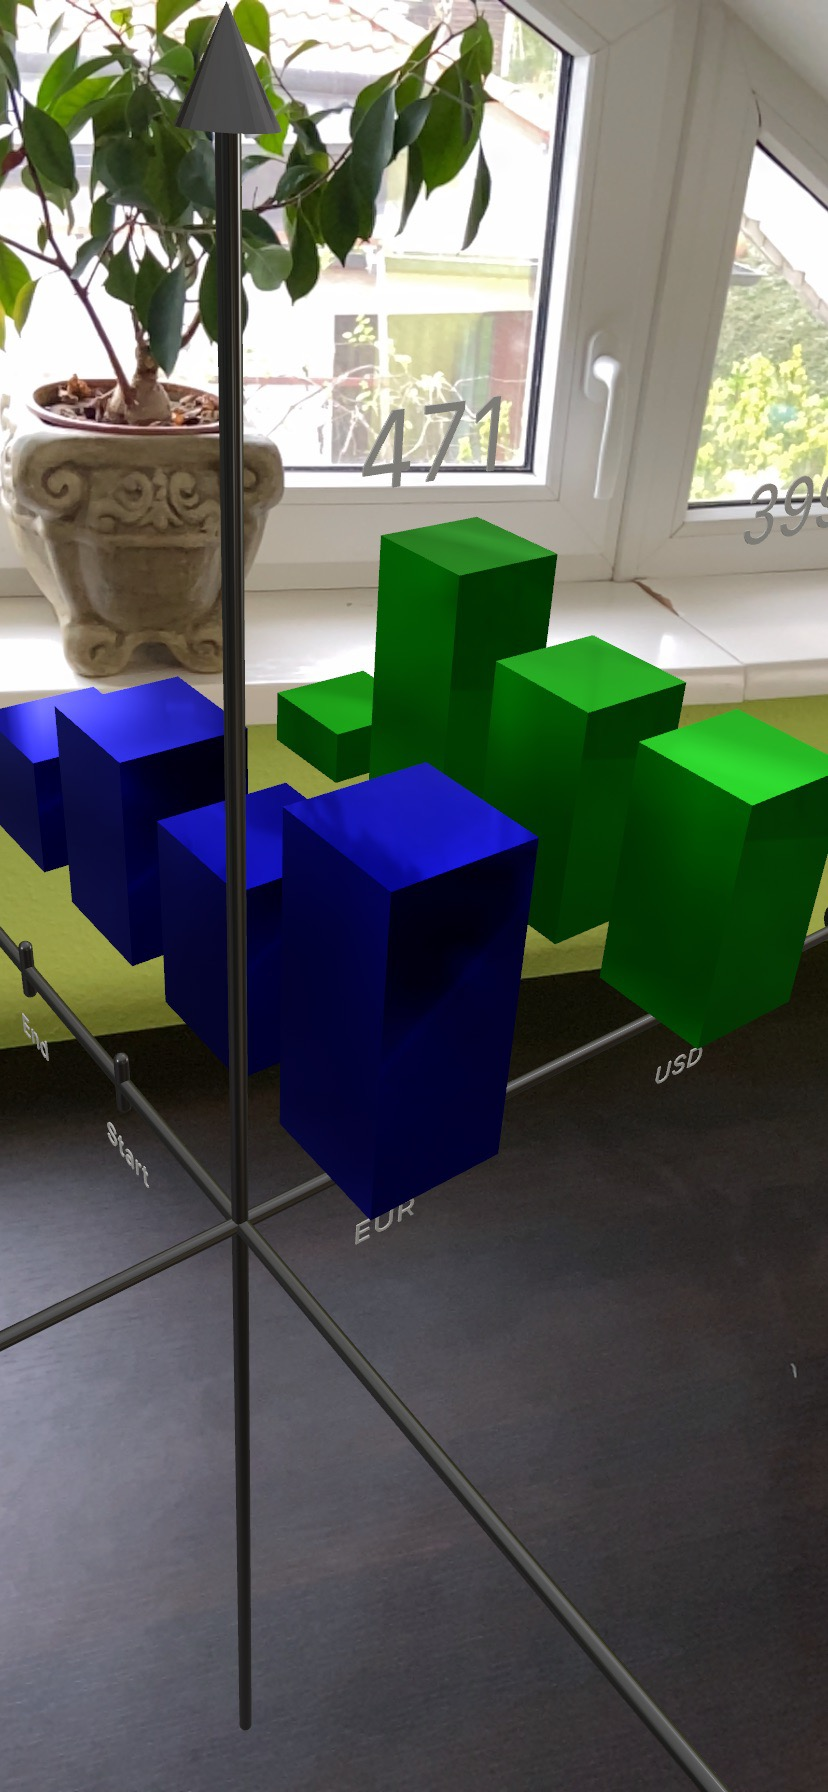
\includegraphics[scale=0.2]{top.jpeg}
  % \includegraphics[width=150mm, keepaspectratio]{figures/TeXnicCenter.png}
  \caption{The main screen of the application.}
  \label{fig:TexnicCenter}
\end{figure}

As the attached images clearly show, the virtual 3D graph can be easily walked around and viewed from different angles, thereby giving users a new comparative perspective. It is possible to move and rotate the entire graph, as well as move the current exchange rate columns to make it easier to compare with other metrics. The move and rotate functions are only available in Spectate mode, for this you have to stop Live mode (or otherwise start Live mode) by pressing the button located in the upper left corner.

Currently, 2 currencies are available in the application, but of course this can be easily expanded at any time in the future. These two are EUR to HUF and USD to HUF. These can be displayed after selection and confirmation from the bottom bar. If the given exchange rate is already placed, it can no longer be added to the graph twice.

\begin{figure}[!ht]
  \centering
  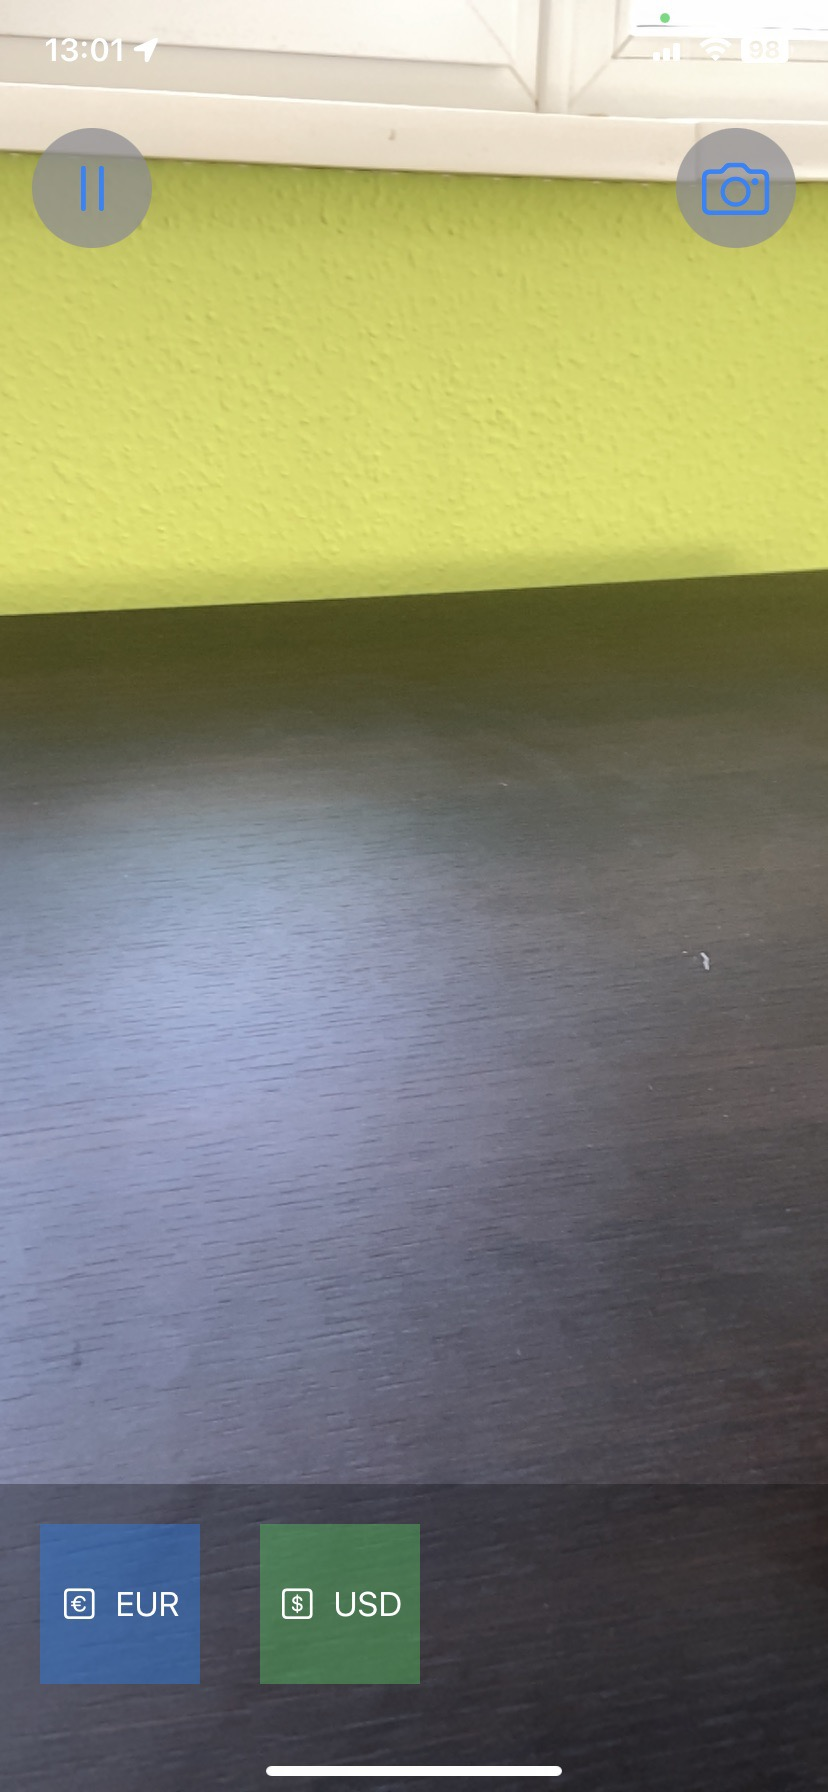
\includegraphics[scale=0.2]{selector.jpeg}
  % \includegraphics[width=150mm, keepaspectratio]{figures/TeXnicCenter.png}
  \caption{The main screen of the application.}
  \label{fig:TexnicCenter}
\end{figure}

\begin{figure}[!ht]
  \centering
  
\includegraphics[scale=0.2]{megerosites.jpeg}
  % \includegraphics[width=150mm, keepaspectratio]{figures/TeXnicCenter.png}
  \caption{The main screen of the application.}
  \label{fig:TexnicCenter}
\end{figure}

\begin{figure}[!ht]
  \centering
  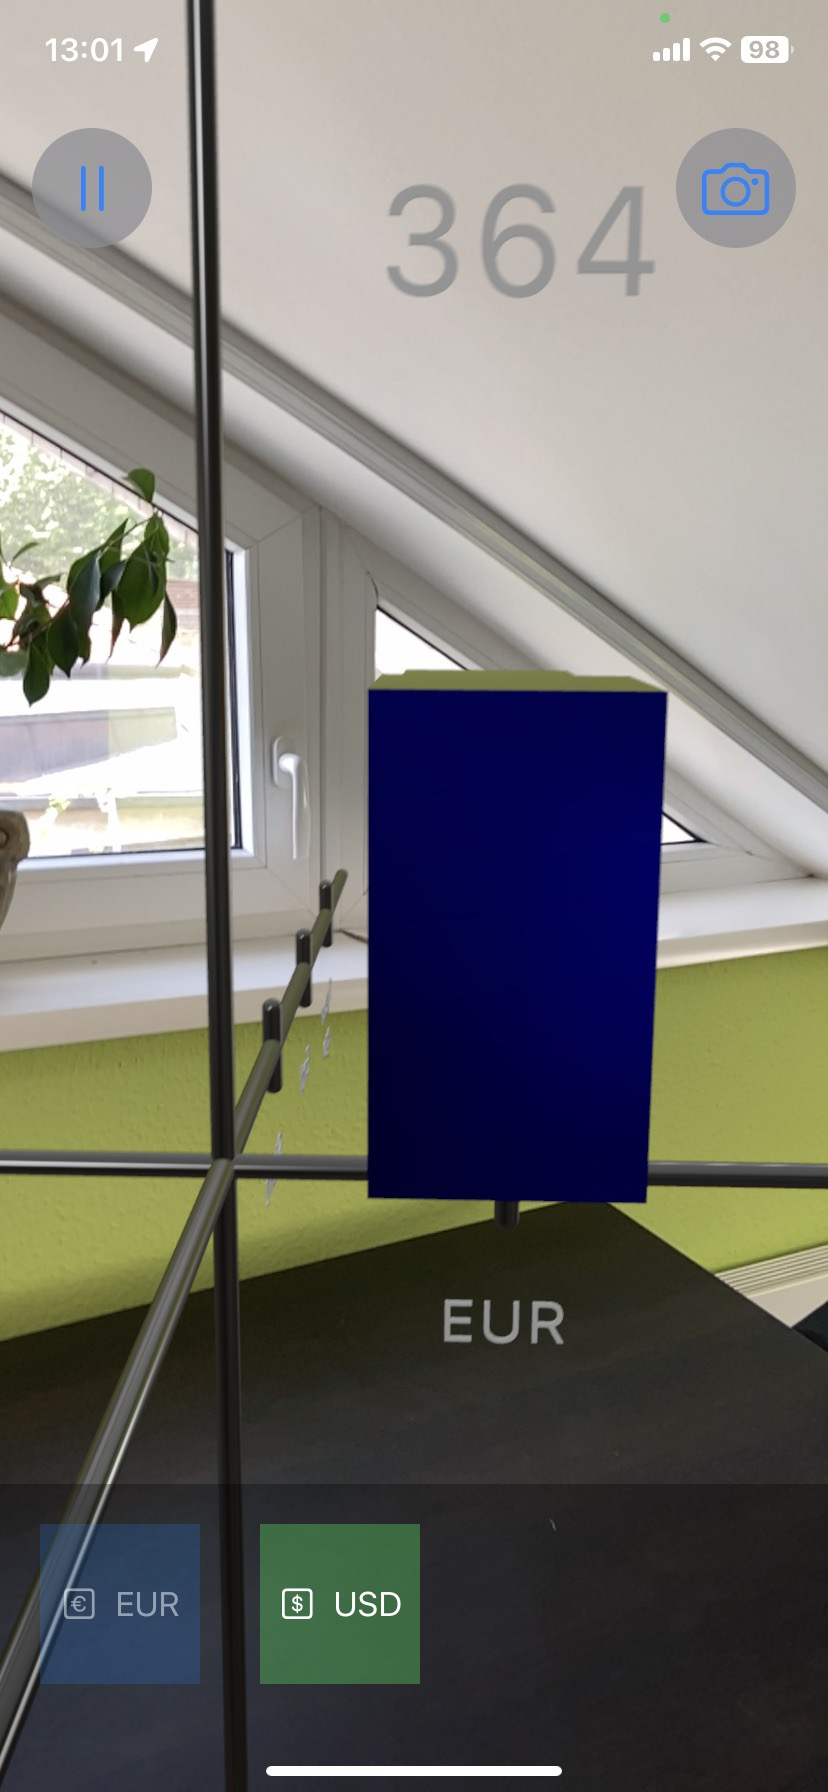
\includegraphics[scale=0.2]{not_available.jpeg}
  % \includegraphics[width=150mm, keepaspectratio]{figures/TeXnicCenter.png}
  \caption{The main screen of the application.}
  \label{fig:TexnicCenter}
\end{figure}





\chapter{Sources}

Below I list the external links and sources used during the project and the report.

% \bibliography{mybib}

%\section{External Links}

\begin{thebibliography}{9}
  \bibitem{techtagaws}
  TechTarget - Amazon Web Services: https://www.techtarget.com/searchaws/definition/Amazon-Web-Services

  \bibitem{lamport94}
  Leslie Lamport (1994) \emph{\LaTeX: a document preparation system}, Addison
  Wesley, Massachusetts, 2nd ed.
\end{thebibliography}

\hyperlink{https://www.techtarget.com/searchaws/definition/Amazon-Web-Services}{TechTarget - Amazon Web Services}

\hyperlink{https://developer.apple.com/augmented-reality/}{Apple - Augmented Reality}

\hyperlink{https://developer.apple.com/documentation/realitykit/}{Apple - RealityKit}

\hyperlink{https://www.kodeco.com/books/apple-augmented-reality-by-tutorials/v1.0/chapters/iii-introduction}{Kodeco - RalityKit tutorials}

\hyperlink{https://developer.apple.com/forums/thread/658300}{Apple Forum - Where to start ARKit}

\hyperlink{https://developer.apple.com/documentation/realitykit/adding-procedural-assets-to-a-scene}{Apple - Adding procedural assets to a scene}

\hyperlink{https://coledennis.medium.com/tutorial-generating-3d-text-with-realitykit-in-a-swiftui-app-fa2a50403012}{Medium - Adding 3D text to scene}

\hyperlink{https://betterprogramming.pub/take-an-arview-snapshot-in-realitykit-93b620cf99b3}{BetterProgramming - Taking AR view snapshot}

\hyperlink{https://www.youtube.com/watch?v=9R_G0EI-UoI}{YouTube - Placing models}

\hyperlink{https://github.com/maxxfrazer/FocusEntity}{GitHub - FocusEntity}

\hyperlink{https://betterprogramming.pub/how-to-add-text-to-an-arview-in-an-ios-application-tutorial-f3f746f4dc1f}{BetterProgramming - Update model entity}

\hyperlink{https://rapidapi.com/apidojo/api/yahoo-finance1}{RapidAPI}

\hyperlink{https://algotrading101.com/learn/yahoo-finance-api-guide/}{Yahoo Financial API Guide}

\hyperlink{https://apilayer.com/marketplace/exchangerates_data-api}{APILayer REST API}

\hyperlink{https://github.com/maxxfrazer/RealityGeometries}{RealityGeometries - Kúpinsta}

\hyperlink{https://www.youtube.com/watch?v=itGRaAryUxA}{YouTube - RealitySchool: Place, Interact with, and Remove AR Objects in RealityKit}

\hyperlink{https://cocoacasts.com/swiftui-fundamentals-what-is-swiftui}{Cocoacast - SwiftUI}

\hyperlink{https://www.hackingwithswift.com/quick-start/swiftui/how-to-use-observedobject-to-manage-state-from-external-objects}{Hacking with Swift - ObservedObject}

\hyperlink{https://developer.mozilla.org/en-US/docs/Glossary/MVC}{Mozilla - MVC}

\end{document}
